\documentclass[12pt]{article}
\usepackage{array}
\usepackage{color}
\usepackage{amsthm}
\usepackage{eufrak}
\usepackage{lipsum}
\usepackage{pifont}
\usepackage{yfonts}
\usepackage{amsmath}
\usepackage{amssymb}
\usepackage{ccfonts}
\usepackage{comment} \usepackage{amsfonts}
\usepackage{fancyhdr}
\usepackage{graphicx}
\usepackage{listings}
\usepackage{mathrsfs}
\usepackage{setspace}
\usepackage{textcomp}
\usepackage{blindtext}
\usepackage{enumerate}
\usepackage{microtype}
\usepackage{xfakebold}
\usepackage{kantlipsum}
%\usepackage{draftwatermark}
\usepackage[spanish]{babel}
\usepackage[margin=1.5cm, top=2cm, bottom=2cm]{geometry}
\usepackage[framemethod=tikz]{mdframed}
\usepackage[colorlinks=true,citecolor=blue,linkcolor=red,urlcolor=magenta]{hyperref}

%//////////////////////////////////////////////////////
% Watermark configuration
%//////////////////////////////////////////////////////
%\SetWatermarkScale{4}
%\SetWatermarkColor{black}
%\SetWatermarkLightness{0.95}
%\SetWatermarkText{\texttt{Watermark}}

%//////////////////////////////////////////////////////
% Frame configuration
%//////////////////////////////////////////////////////
\newmdenv[tikzsetting={draw=gray,fill=white,fill opacity=0},backgroundcolor=none]{Frame}

%//////////////////////////////////////////////////////
% Font style configuration
%//////////////////////////////////////////////////////
\renewcommand{\familydefault}{\ttdefault}
\renewcommand{\rmdefault}{tt}

%//////////////////////////////////////////////////////
% Bold configuration
%//////////////////////////////////////////////////////
\newcommand{\fbseries}{\unskip\setBold\aftergroup\unsetBold\aftergroup\ignorespaces}
\makeatletter
\newcommand{\setBoldness}[1]{\def\fake@bold{#1}}
\makeatother

%//////////////////////////////////////////////////////
% Default font configuration
%//////////////////////////////////////////////////////
\DeclareFontFamily{\encodingdefault}{\ttdefault}{%
  \hyphenchar\font=\defaulthyphenchar
  \fontdimen2\font=0.33333em
  \fontdimen3\font=0.16667em
  \fontdimen4\font=0.11111em
  \fontdimen7\font=0.11111em}



\begin{document}
    %//////////////////////////////////////////////////////
% Heading Configuration
%//////////////////////////////////////////////////////
\pagestyle{fancy}
\thispagestyle{plain}
\fancyhead[RO,L]{\textbf{Teoria de Grafos}}
\fancyhead[LO,L]{\textbf{Tarea 2}}
\setlength{\headheight}{16.0pt}

%//////////////////////////////////////////////////////
% Subsections Configuration
%//////////////////////////////////////////////////////
\renewcommand*\thesubsection{\arabic{subsection}}
\newcounter{counter}
\newlength{\palabra}
\settowidth{\palabra}{counter 999.}
\newcommand{\makeboxlabel}[1]{\fbox{#1.}\hfill}

%//////////////////////////////////////////////////////
% Personalized commands configuration
%//////////////////////////////////////////////////////
\newcommand{\N}{\mathbb{N}}
\newcommand{\Z}{\mathbb{Z}}
\newcommand{\Q}{\mathbb{Q}}
\newcommand{\R}{\mathbb{R}}
\newcommand{\C}{\mathbb{C}}
\newcommand{\re}{\operatorname{Re}}
\newcommand{\im}{\operatorname{Im}}
\newcommand{\Aut}{\operatorname{Aut}}
\newcommand{\GCD}{\operatorname{GCD}}
\newcommand{\LCD}{\operatorname{LCD}}
\linespread{1} %Line spacing

%//////////////////////////////////////////////////////
% Inline code configuration
%//////////////////////////////////////////////////////
\lstset{
gobble=5,
numbers=left,
frame=single,
framerule=1pt,
showtabs=False,
showspaces=False,
showstringspaces=False,
backgroundcolor=\color{gray}}

%//////////////////////////////////////////////////////
% Problem list configuration
%//////////////////////////////////////////////////////
\newenvironment{problems}
  {\begin{list}
     {{\fbseries Problem \arabic{counter}.}}
    {\usecounter{counter}
     \setlength{\labelsep}{1em}
     \setlength{\itemsep}{2pt}
     \setlength{\leftmargin}{2em}
     \setlength{\rightmargin}{0cm}
     \setlength{\itemindent}{1em} }}
{\end{list}}

%//////////////////////////////////////////////////////
% Appendix configuration
%//////////////////////////////////////////////////////
\newenvironment{Appendix}
  {\begin{list}
     {{\fbseries Lemma \arabic{counter}.}}
    {\usecounter{counter}
     \setlength{\labelsep}{1em}
     \setlength{\itemsep}{2pt}
     \setlength{\leftmargin}{2em}
     \setlength{\rightmargin}{0cm}
     \setlength{\itemindent}{1em} }}
{\end{list}}

%//////////////////////////////////////////////////////
% Notes configuration
%//////////////////////////////////////////////////////
\newenvironment{notes}
  {\begin{list}
     {{\fbseries Note \arabic{counter}.}}
    {\usecounter{counter}
     \setlength{\labelsep}{1em}
     \setlength{\itemsep}{2pt}
     \setlength{\leftmargin}{2em}
     \setlength{\rightmargin}{0cm}
     \setlength{\itemindent}{1em} }}
{\end{list}}

%//////////////////////////////////////////////////////
% Activity Information
%//////////////////////////////////////////////////////
\vspace*{-1cm}
\hrule width \hsize \kern 1mm \hrule width \hsize height 2pt
\begin{center}
   \parbox[c]{.32\textwidth}{
   \hspace{1cm}\\
   Sergio Montoya Ramirez\\
   202112171}
%   Luis Ernesto Tejón Rojas\\
%   202113150}
   \hspace*{\fill}
   \parbox[c]{.35\textwidth}{\centering
   Universidad de Los Andes\\
   Tarea 1\\
   Teoria de Grafos\\
   }
   \hspace*{\fill}
   \parbox[c]{.3\textwidth}{
   \begin{flushleft}
      Bogotá D.C., Colombia\\
      \today
   \end{flushleft}}
\end{center}
\hrule width \hsize height 2pt \kern 1mm \hrule width \hsize

\bigskip

\bigskip


    \begin{enumerate}
      \item tenemos la función: \[
	  f\left( x \right) =
      \begin{cases}
	V_0 &\ 0 < x \le 1\\
	-V_0 & -1 \le x < 0
      \end{cases}
      .\] 
      Decimos entonces que la expresión de $f$ en polinomios de Legendre es: \[
      f\left( x \right) = \displaystyle \sum_{n=0}^{\infty} a_nP_n\left( x \right) 
      .\] Donde los coeficientes están determinados por:
      \begin{align*}
	a_n &= \frac{2n + 1}{2} \int_{-1}^{1} f\left( x \right) P_n\left( x \right) dx \\
	    &= \frac{2n + 1}{2} \left[ \int_{-1}^{0} \left( -V_{0} \right) P_n dx + \int_{0}^{1}V_0P_n dx \right]\\
	    &= \frac{2n + 1}{2}V_0 \left[ \int_{0}^{1}P_n\left( x \right) dx - \int_{-1}^{0}P_n\left( x \right) dx \right] 
      .\end{align*}

      Ahora bien, se tienen dos casos, $P_n$ par o impar:
      \begin{itemize}
        \item Para $P_n$ impar, $P_n\left( -x \right) = - P_n\left( x \right) \implies \int_{-1}^{0} P_n\left( x \right) dx = - \int_0^{1}P_n\left( x \right) dx$
	\item Para $P_n$ par, $P_n\left( -x \right) = P_n\left( x \right) \implies \int_{-1}^{0}P_n\left( x \right) dx = \int_0^{1} P_n\left( x \right) dx$
      \end{itemize}
      Con lo cual que podemos ver que los términos pares se contrarrestan. Por lo cual, tenemos que: \[
	a_n = \frac{2n + 1}{2}V_0 \left[ \int_0^{1}P_n\left( x \right) dx - \int_{-1}^{0}P_n\left( x \right) dx \right] = \left( 2n + 1 \right) V_0 \int_0^{1}P_n\left( x \right) dx
      .\] Luego: \[
      f\left( x \right)  = \sum_{n=0}^{\infty} \left( 2n + 1 \right) V_0 \int_{0}^{1}P_n\left( x \right) dx P_n\left( x \right) 
      .\] Ademas, recordemos que $P_n$ es impar. Con esto entonces calculemos:
      \begin{align*}
	\int_{0}^{1} P_1 \left( x \right) dx &= \int_{0}^{1}x dx = \frac{x^2}{2} |_{0}^{1} = \frac{1}{2}\\
	\int_{0}^{1}P_3\left( x \right) dx &= \int_{0}^{1}\frac{1}{2}\left( 5x^{3}- 3x \right) dx\\
	&=  \frac{1}{2}\left[ \frac{5x^{4}}{4} - \frac{3x^2}{2} \right]_0^{1}\\
	&= \frac{1}{4}\left( \frac{5}{2} - 3 \right)  \\
	\implies& f\left( x \right) = \frac{3}{2}V_0 x - \frac{7}{8}V_0\left( 5x^{3}- 3x \right) + \ldots
      .\end{align*}
    \item Para comenzar en este caso seria prudente darnos una idea de las ubicaciones con las que estamos trabajando. Si hacemos un gráfico con la descripción dada en el enunciado nos queda:
      \begin{figure}[h]
        \centering
        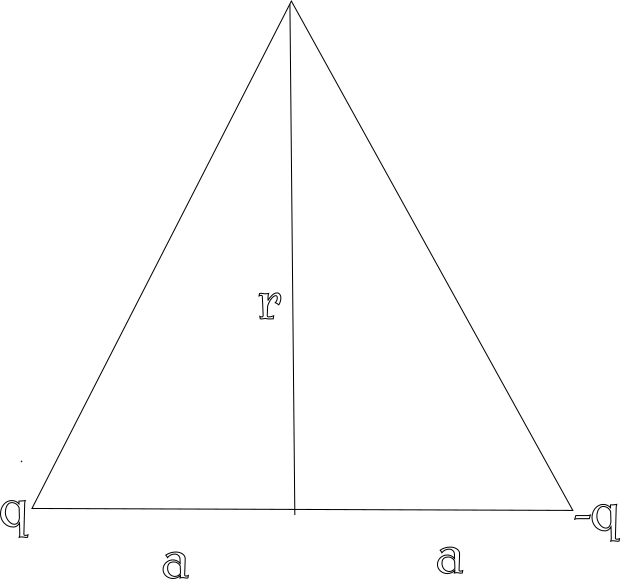
\includegraphics[width=0.3\textwidth]{Imagenes/punto_2.png}
        \caption{Imagen que gráfica el caso descrito por el enunciado del punto.}
        \label{fig:punto_2}
      \end{figure}

      Como podemos ver en la imagen \label{fig:punto_2} la distancia que hay desde el punto que se nos solicita a ambos otros puntos es básicamente la misma. Esta distancia, la podemos encontrar por medio del teorema de pitagoras:
      \begin{align*}
        h^2 &= c_1^2 + c_2^2 \\
	h^2 &= a^2 + r^2 \\
	h &= \sqrt{a^2 + r^2}  \\
      .\end{align*}

      Donde $h$ es la distancia que hay en ambos casos. Ahora bien recordemos que el potencial eléctrico para un punto $p$ con varias fuentes puntuales es: \[
	V_p = \displaystyle\sum_{n = 1}^{N} V_n
      .\] 

      Donde $V_n$ es el potencial de cada una de las fuentes puntuales. Ahora bien, con esto entonces calculemos $V$ con:  \[
      V = \frac{kq}{r}
      .\] con lo cual esto nos queda:
      \begin{align*}
        V = \frac{k q}{\sqrt{a^2 + r^2} } - \frac{k q}{\sqrt{a^2 + r^2} }
      .\end{align*}

      Pero este es un resultado que es solo valido para cuando la distancia que mantiene es la misma. Sin embargo intentemos describirlo para cuando las distancias son distintas. Podemos mostrar que es:
      \begin{align*}
        V_p &= V_{+} + V_{-} = kq\left( \frac{1}{r_+} - \frac{1}{r_-} \right)  \\
	r_{\pm} &= \sqrt{x^2 + \left( y \mp \frac{d}{2} \right)^2 } 
      .\end{align*}

      Ya con esto describimos el potencial para cualquier punto. Sin embargo ahora desarrollemos el hecho de que $r \gg a$.

      Podemos reescribir los radios en términos polares. Es decir, $x = r \sin\left( \theta \right) $ y $y = r \cos\left( \theta \right) $ con lo cual nos queda:
      \begin{align*}
        r_{\pm} &= \sqrt{r^2\sin^2\left( \theta \right) + \left( r \cos\left( \theta \right) \mp \frac{a}{2} \right)^2}  \\
	r_{\pm} &= r \sqrt{\sin^2\left( \theta \right)  + \left( \cos\left( \theta \right) \mp \frac{a}{2r} \right)^2 }  \\
	r_{\pm} &= r \sqrt{\sin^2\left( \theta \right) + \cos^2\left( \theta \right) \mp \cos\left( \theta \right) \frac{a}{r} + \left( \frac{a}{2r} \right)^2 }  \\
	&= r \sqrt{1 \mp \cos\left( \theta \right) \frac{a}{r} + \left( \frac{a}{2r} \right)^2}  \\
      .\end{align*}

      Ahora bien, dado que $r \gg a$ entonces el termino $\frac{a}{2r}$ es extremadamente pequeño y al hacer $\left( \frac{a}{2r} \right)^2$ es esencialmente 0. Con lo cual queda:
      \begin{align*}
        r_{\pm} &= r \sqrt{1 \mp \cos\left( \theta \right) \frac{d}{r}}  \\
	\frac{1}{\sqrt{1 \pm \alpha} } &\approx 1 \pm \frac{\alpha}{2}\\
        V_p &= V_{+} + V_{-} = kq\left( \frac{1}{r_+} - \frac{1}{r_-} \right)  \\
        V_p &= kq\left( \frac{1}{r \sqrt{1 + \cos\left( \theta \right) \frac{d}{r}}} - \frac{1}{r \sqrt{1 - \cos\left( \theta \right) \frac{d}{r}}} \right)  \\
	V_p &= \frac{kq}{r} \left(\left( 1 + \frac{d\cos\left( \theta \right) }{2r} \right) - \left( 1 - \frac{d\cos\left( \theta \right) }{2r} \right)  \right)  \\
	&= k \frac{qd\cos\left( \theta \right) }{r^2} \\
      .\end{align*}

    \item Suponemos que \[
    f\left( \rho \right) = \sum_{n=1}^{\infty} A_{v_n} J_v\left[ X_{v_n}\frac{\rho}{b} \right] 	
    .\] con
    \begin{align*}
      A_{v_n} &= \frac{2}{b^2\left[ J_{v + 1}\left( X_{v_n} \right) \right]^2}\int_{0}^{b}\rho\left( \rho^{k} \right) J_v\left( X_{v_n}\frac{\rho}{b} \right) d\rho\\
      \frac{d\left[ Y^{n}J_n \right] }{dy} &= Y^{n}J_{n - 1}\\
      A_{v_n} &= \frac{2}{b^2\left[ J_{v + 1}\left( X_{v_n} \right) \right]^2}\int_{0}^{b}\left( \rho^{k + 1} \right) J_v\left( X_{v_n}\frac{\rho}{b} \right) d\rho\\
      Y &= X_{v_n}\frac{\rho}{b} \\
      \frac{dY}{d\rho} &= \frac{X_{v_n}}{b} \leftrightarrow d\rho = \frac{b}{X_{v_n}} \\
      \rho &= \frac{Y b}{X_{v_n}} \\
      A_{v_n} &= \frac{2}{b^2\left[ J_{v + 1}\left( X_{v_n} \right)  \right]^2}\int_0^{X_{v_n}}\left( \frac{yb}{X_{v_n}} \right)^{k + 1}J_{v}\left( y \right) \frac{b}{x_{v_n}}dY\\
	      &= \frac{2}{b^2 \left[ J_{v+1}\left( X_{v_n} \right)  \right]^2}\int_{0}^{X_{v_n}}\frac{y^{k + 1}b^{k + 2}}{X_{v_n}^{k + 2}}J_v\left( Y \right) dY \\
	      &= \frac{2b^{k}}{\left[ J_{v+1}\left( X_{v_n} \right)  \right]^2 X_{v_n}^{(k + 2)} }\int_0^{X_{v_n}}Y^{k + 1}J_v\left( Y \right) dY \\
    \end{align*}
    Si $v = k$
    \begin{align*}
      \frac{d\left[ Y^{k}J_k\left( v \right)  \right] }{dY} &= Y^{k + 1}J_{k}\left( V \right)  \\
      A_{k_n} &= \frac{2b^{k}}{\left[ J_{v+1}\left( X_{v_n} \right)  \right]^2 X_{v_n}^{(k + 2)} }\int_0^{X_{v_n}}Y^{k + 1}J_v\left( Y \right) dY \\
      &= \frac{2b^{k}}{\left[ J_{v+1}\left( X_{v_n} \right)  \right]^2 X_{v_n}^{(k + 2)} }\left[ Y^{k}J_k\left( Y \right) \right]_0^{X_{k_n}}\\
      &=  \frac{2b^{k}}{\left[ J_{v+1}\left( X_{v_n} \right)  \right]^2 X_{v_n}^{(k + 2)} }  \left[ X_{k_n}^{k}J_k\left( x_{k_n} \right) - 0 \right] \\
      &= \frac{2b^{k}}{\left[ J_{v+1}\left( X_{v_n} \right)  \right]^2 X_{v_n}^{(k + 2)} } \frac{J_k\left( X_{k_n} \right) }{X^2_{k_n}} \\
      f\left( \rho \right) &= \rho^{k} = \sum_{n=1}^{\infty} \frac{2b^{k}}{\left[ J_{v+1}\left( X_{v_n} \right)  \right]^2 X_{v_n}^{(k + 2)} }\frac{J_k\left( X_{k_n} \right) }{X^2_{k_n}} J_k \left[ X_{k_n} \frac{\rho}{b} \right] 
    .\end{align*}
    \item Para este caso
    \item 
      \begin{enumerate}
        \item En este caso partimos de que 
      \end{enumerate}
    \end{enumerate}
\end{document}
